\documentclass[nofootinbib,amssymb,amsmath]{revtex4}
\usepackage{mathtools}
\usepackage{amsthm}
\usepackage{algorithm}
\usepackage{algpseudocode}
\usepackage{lmodern}
\usepackage{graphicx}
\usepackage{color}

%Put an averaged random variable between brackets
\newcommand{\ave}[1]{\left\langle #1 \right\rangle}

\newcommand{\vzero}{{\bf 0}}
\newcommand{\vI}{{\bf I}}
\newcommand{\vb}{{\bf b}}
\newcommand{\vd}{{\bf d}}
\newcommand{\vc}{{\bf c}}
\newcommand{\vv}{{\bf v}}
\newcommand{\vz}{{\bf z}}
\newcommand{\vn}{{\bf n}}
\newcommand{\vm}{{\bf m}}
\newcommand{\vG}{{\bf G}}
\newcommand{\vQ}{{\bf Q}}
\newcommand{\vM}{{\bf M}}
\newcommand{\vW}{{\bf W}}
\newcommand{\vX}{{\bf X}}
\newcommand{\vPsi}{{\bf \Psi}}
\newcommand{\vSigma}{{\bf \Sigma}}
\newcommand{\vlambda}{{\bf \lambda}}
\newcommand{\vLambda}{{\bf \Lambda}}
\newcommand{\vA}{{\bf A}}
\newcommand{\MM}{M}
\newcommand{\PP}{\mathcal{P}}
\newcommand{\EE}{\mathbb{E}}
\newcommand{\norm}{{\mathcal N}}

\newtheorem{lemma}{Lemma}
\newtheorem{corollary}{Corollary}

\def\SL#1{{\color [rgb]{0,0,0.8} [SL: #1]}}
\def\DB#1{{\color [rgb]{0,0.8,0} [DB: #1]}}

\newcommand{\HOM}{$\mathsf{Hom}$}
\newcommand{\HET}{$\mathsf{Het}$}
\newcommand{\REF}{$\mathsf{Ref}$}
\newcommand{\epss}{\varepsilon}

\makeatletter
\DeclareFontFamily{OMX}{MnSymbolE}{}
\DeclareSymbolFont{MnLargeSymbols}{OMX}{MnSymbolE}{m}{n}
\SetSymbolFont{MnLargeSymbols}{bold}{OMX}{MnSymbolE}{b}{n}
\DeclareFontShape{OMX}{MnSymbolE}{m}{n}{
    <-6>  MnSymbolE5
   <6-7>  MnSymbolE6
   <7-8>  MnSymbolE7
   <8-9>  MnSymbolE8
   <9-10> MnSymbolE9
  <10-12> MnSymbolE10
  <12->   MnSymbolE12
}{}
\DeclareFontShape{OMX}{MnSymbolE}{b}{n}{
    <-6>  MnSymbolE-Bold5
   <6-7>  MnSymbolE-Bold6
   <7-8>  MnSymbolE-Bold7
   <8-9>  MnSymbolE-Bold8
   <9-10> MnSymbolE-Bold9
  <10-12> MnSymbolE-Bold10
  <12->   MnSymbolE-Bold12
}{}

\let\llangle\@undefined
\let\rrangle\@undefined
\DeclareMathDelimiter{\llangle}{\mathopen}%
                     {MnLargeSymbols}{'164}{MnLargeSymbols}{'164}
\DeclareMathDelimiter{\rrangle}{\mathclose}%
                     {MnLargeSymbols}{'171}{MnLargeSymbols}{'171}
\makeatother

\begin{document}

\title{Notes on CNV Methods}
\author{Samuel K. Lee}
\email{slee@broadinstitute.org}
\affiliation{Broad Institute, 75 Ames Street, Cambridge, MA 02142}

\author{David Benjamin}
\email{davidben@broadinstitute.org}
\affiliation{Broad Institute, 75 Ames Street, Cambridge, MA 02142}

\author{Mehrtash Babadi}
\email{mehrtash@broadinstitute.org}
\affiliation{Broad Institute, 75 Ames Street, Cambridge, MA 02142}

\date{\today}

\begin{abstract}
Some notes on current and proposed methods used in the GATK CNV and ACNV workflows.
\end{abstract}

\maketitle

\section{Introduction}\label{introduction}

The GATK uses two types of information from sequencing data to detect copy number variations (CNVs).  First, targets (usually exons but in principle any genomic locus) with abnormally high or low coverage suggest amplifications or deletions, respectively.  Second, sites that are heterozygous in a normal sample and have allele ration significantly different from 1:1 in the matched tumor sample imply a CNV event involving one or both alleles.  The workflow is as follows:

\begin{enumerate}

\item Partition targets into continuous segments that represent the same copy-number event using coverage data.  The segmentation is performed by a circular-binary-segmentation (CBS) algorithm described by Olshen et al. 2004 that was originally developed to segment noisy array copy-number data.\footnote{Specifically, the CBS implementation provided by the \texttt{R} package \texttt{DNACopy} is used.}

\item Find heterozygous sites in the normal case sample and segment these, again using CBS, according to their ref:alt allele ratios in the tumor sample.

\item Combine the two sets of segments in a liberal manner that tends to produce too many segments.

\item Alternate between modeling the copy ratio and minor allele fraction of each segment with merging adjacent segments that are sufficiently similar according to this model.

\end{enumerate}

\section{Segmentation by Coverage and Minor Allele Fraction} \label{recapseg-overview}

\subsection{Panel of Normals}
We cannot simply divide the coverage of each target by the average sequencing depth to obtain an estimate of its copy ratio.  The coverage of different targets is heavily-biased by factors including the efficiency of their baits, GC content, and mappability.  In order to detect CNVs we must model the coverage of each target in the absence of CNVs, which requires a panel of normal samples (PoN) that are representative of the sequencing conditions of the case sample.  PoN samples must be created using the same baits as the case sample.  The steps for creating a panel of normals are

\begin{enumerate}

\item  Obtain the coverage (total number of overlapping reads) of every target and sample.

\item Calculate the median coverage of each target over all samples.

\item  Filter out targets whose median coverage is below a given percentile (by default 25\%) of target medians.

\item  Divide all coverages by their corresponding target medians.

\item Filter out samples with too great a proportion of zero-coverage targets (by default 5\%).

\item Filter out targets with zero coverage in too great a proportion of samples (by default 2\%).

\item Filter out samples whose median coverage is above or below certain percentiles (by default 2.5\% and 97.5\%) of sample medians.

\item Replace all remaining zero coverages with their corresponding target median. 

\item Calculate the range of coverage from percentile $p$\% to $(100 - p)$\% for each target and truncate coverages at each target to lie within these ranges.  By default $p = 0.1$.

\item Divide each coverage by its sample median.

\item Take the $\log_2$ of each coverage.

\item Calculate the median of each sample and take the median of these over all targets.  Subtract this median of medians from each coverage.

\item Perform a singular value decomposition (SVD) of the resulting matrix and calculate its pseudo-inverse truncated to the space spanned by the $k$ right eigenvectors with largest singular values. Choose $k$ using Jollife's heuristic of retaining singular values greater than 0.7 times the mean singular value.

\end{enumerate}

The output is: a $N \times k$ matrix $P$, the columns of which are the the retained right eigenvectors (eigensamples), and its pseudoinverse $P^+$; and the target medians (before any transformations).  Here $N$ denotes the number of targets.

\subsection{Segmentation by tangent-normalized coverage}
We first divide the integer coverage of the case sample at each target by the corresponding target median from the PoN and take the $\log_2$ transformation to obtain an $N \times 1$ column matrix ${\bf x}$.  We then calculate the ``tangent-normalized'' coverage: ${\bf x} - PP^+ {\bf x}$.  The meaning of this is as follows: $PP^+$ is an operator that projects onto the column space of $P$.  That is, it projects onto the space spanned by the $k$ most significant eigensamples representing the (non-CNV-related) variability of the coverage.  Subtracting the projection $PP^+ {\bf x}$ therefore isolates the CNV signal and removes noise due to fluctuations in sequencing bias.

Finally, the tangent-normalized coverage vector is passed to CBS to obtain coverage segments.

\subsection{Het coverage and segmentation by minor allele fraction}
Given a large database of common SNPs, we search the normal control sample for heterozygous sites.  To determine whether a site with $r$ ref reads and $a$ alt reads is heterozygous, we calculate the two-sided $p$-value under the null hypothesis that the number of alt reads follows a binomial distribution: $a \sim {\rm Binom}(a + r, 1/2)$.  If the $p$-value is not too small we consider the site heterozygous.

Ref and alt counts are then obtained at these sites in the tumor case sample.  To obtain initial minor-allele-fraction segments, we estimate the minor allele fraction for each het site by taking the maximum-likelihood estimate given by Equation~\ref{likelihood} with allelic bias ignored (i.e., $\lambda_j = 1$) and pass the resulting list to CBS.

\subsection{Target/SNP segment union} \label{targetsnp-segment-union}

\SL{SL will fill this in.}

\subsection{Small-segment merging} \label{small-segment-merging}

\SL{SL to update this to the new method.}

Using CBS to segment the targets in GATK CNV results in segments that are larger than a specified minimum number of targets $n_t$ (by default, $n_t = 2$).  However, after taking the union of target and SNP segments, small segments with less than $n_t$ targets may be introduced.  To be consistent with CBS and CNV, ACNV treats these small segments as spurious, and removes them by merging them with adjacent segments.

\subsection{A Bayesian model for detecting Heterozygous sites}
Here, we would like to propose a slightly different scheme for calling Heterozygous (\HET) sites that (1) takes into account the base read alignment and sequencing qualities, and (2) works for both normal and tumor data. Provisioning situations that only the tumor data is available to us (``tumor-only''), in addition to the presently cosindered situation of paired normal-tumor data (``paired normal-tumor''), we need to modify our criterion for calling a \HET~site. Conceptually, since reads from tumor samples are not pure (contaminated with subclones, normals, etc), a statistical test that rejects the \HET~hypothesis based on the premise of having equal probability of $\mathsf{Ref}$ and $\mathsf{Alt}$ reads is bound to reject \HET~cases when applied to tumor reads. Here, we propose a more sensible Bayesian model.\\

\noindent {\bf Notation:} Let us first focus on a single site $j$, with $R_{kj} \in \{A, C, T, G\}$ denoting the mapped base at site $j$ from read $k$, and $\varepsilon^B_{kj}$ and $\varepsilon^M_k$ denoting the err probability of base calling and mapping. Also, let $\mathsf{Ref}_j$ and $\mathsf{Alt}_j$ denote the Ref and Alt alleles at this site.\\

\noindent{\bf Definition of error:} In case of a base error event, the base could be read as any other three bases with equal probability. In case of a mapping error event, we assume equal probability for all four bases.\\

\noindent{\bf Rareness of somatic SNP events:} In order to proceed with the model, we assume that somatic SNPs are rare events such that Hom/Het sites retain their germline identity.\\

\noindent{\bf Likelihood of \HOM$_j$:} Assuming that site $j$ is \HOM, we find the likelihood of the reads by conditioning over the allele and error events. We easily find:
\begin{multline}
P(R_{kj}|\mathsf{Hom}_j) = P(\mathsf{Ref}_j|\mathsf{Hom}_j)\prod_{k=1}^{N_j}\left[\frac{\epss^B_{kj}}{3} + \frac{\epss^M_{k}}{4} + \left(1 - \frac{4}{3}\,\epss^B_{kj} - \epss^M_k\right)\delta_{R_{kj}, \mathsf{Ref}_j}\right] +\\
P(\mathsf{Alt}_j|\mathsf{Hom}_j)\prod_{k=1}^{N_j}\left[\frac{\epss^B_{kj}}{3} + \frac{\epss^M_{k}}{4} + \left(1 - \frac{4}{3}\,\epss^B_{kj} - \epss^M_k\right)\delta_{R_{kj}, \mathsf{Alt}_j}\right].
\end{multline}
We need to know the two priors $P(\mathsf{Ref}_j|\mathsf{Hom}_j)$ and $P(\mathsf{Alt}_j|\mathsf{Hom}_j)$, both of which can be estimation from the statistics of the population to which the sample belongs. If this data is not available, we may use the flat prior $P(\mathsf{Ref}_j|\mathsf{Hom}_j) = P(\mathsf{Alt}_j|\mathsf{Hom}_j) = 1/2$ with little harm. \\

\noindent{\bf Likelihood of \HET$_j$:} Assuming that site $j$ is \HET, and that the the probability of the Ref allele in the sample is $f_{j,R}$, we have:
\begin{align}
p_{kj,R} &\equiv P(R_{kj} = \mathsf{Ref}_j| \mathsf{Het}_j, f_{j,R}) = (1-\epss^B_{kj} - \epss^M_k)\,f_{j,R} + \frac{\epss^B_{kj}}{3}\,(1-f_{j,R}) + \epss^M_k/4,\nonumber\\
p_{kj,A} &\equiv P(R_{kj} = \mathsf{Alt}_j| \mathsf{Het}_j, f_{j,R}) = (1-\epss^B_{kj} - \epss^M_k)\,(1-f_{j,R}) + \frac{\epss^B_{kj}}{3}\,f_{j,R} + \epss^M_k/4,\nonumber\\
p_{kj,\circ} &\equiv P(R_{kj} \neq \mathsf{Ref}_j, \mathsf{Alt}_j| \mathsf{Het}_j, f_{j,R}) = \frac{\epss^B_{kj}}{3} + \frac{\epss^M_{k}}{4}.
\end{align}
Therefore, the likelihood reads:
\begin{equation}
P(\{R_{kj}\}|\mathsf{Het}_j) = \int_0^1 \mathrm{d} f_{j,R}\,P(f_{j,R}|\mathsf{Het}_j) \, \prod_{k=1}^{N_j} p_{kj,R}^{I(R_{kj}=\mathsf{Ref}_j)} \, p_{kj,A}^{I(R_{kj}=\mathsf{Alt}_j)}\,p_{kj,\circ}^{I(R_{kj} \neq \mathsf{Ref}_j, \mathsf{Alt}_j)}.
\end{equation}

The integration over $f_{R,j}$ is not as trivial as before since (1) the error probabilities differs from site to site, and (2) the prior is not necessary conjugate to \HET~likelihood. For the uniformity of notation, we define:
\begin{align}
R_{kj} = \mathsf{Ref}_j \quad &\Rightarrow \quad \alpha_{kj} \equiv \frac{\epss^B_{kj}}{3} + \frac{\epss^M_{k}}{4}, \quad \beta_{kj} = 1 - \frac{4\,\epss^B_{kj}}{3} - \frac{\epss^M_k}{4},\nonumber\\
R_{kj} = \mathsf{Alt}_j \quad &\Rightarrow \quad \alpha_{kj} \equiv 1 - \varepsilon^B_{kj} - \frac{3\,\epss^M_k}{4}, \quad \beta_{kj} = -1 + \frac{4 \, \epss^B_{kj}}{3} + \epss^M_k.
\end{align}
such that:
\begin{equation}\label{eq:Phet}
P(\{R_{kj}\}|\mathsf{Het}_j) = \left[\prod_{k \in \mathcal{I}_\circ} \frac{\varepsilon_{kj}}{3}\right]\left[\int_0^1 \mathrm{d} f \, P(f|\mathsf{Het})\, \prod_{k \in \mathcal{I}_{RA}}(\alpha_{kj} + \beta_{kj} f)\right],
\end{equation}
where $\mathcal{I}_\circ$ are the indices of reads that are neither Ref or Alt at site $j$, and $\mathcal{I}_{RA}$ are indices of reads that either Ref or Alt. Furthermore, $P(f|\mathsf{Het})$ is the common prior for Ref allele fraction. For a given prior, we calculate the $f$-integral numerically with a fixed-order quadrature. Since the integrand is polynomial of $f$, a Gaussian quadrature is well-suited to approximate the integral provided that the prior is also smooth.\\

\noindent {\bf Caveats:} (1) sensitivity to error underestimation: if the read/alignment qualities are overestimated, even a single deviation from the $\mathsf{Hom}_j$ hypothesis can dramatically reduce the likelihood. (2) Loss of heterozygosity can manifest itself has homozoygosity; in practice, it should not be an issue since the samples are not pure and germline heterozygosity should yield sufficient evidence to reject the Hom hypothesis. (3) Heterozygosity in a sizable subclone resulting from a somatic SNP may manifest itself as germline heterozygosity. This is also expected not to be a major issue since somatic SNPs are rare.\\


\noindent {\bf A model prior for allele fraction at Het sites:} In this section, we construct a simple prior for the Ref allele fraction at Het sites. To this end, we assume (1) a minimum (maximum) fraction $\rho_\mathrm{min}$ ($\rho_\mathrm{max}$) of the cells in the sample may have events that change the allele fraction with respect to germline (large copy number events, CNLOH, etc). Furthermore, we assume that the maximum copy number is bounded from above by $N_c$. Otherwise, we assume flat priors over both the copy number and non-germline fraction. Under these assumptions, the distribution of the Ref allele fraction is given by:
\begin{equation}
P(f|\mathsf{Het}) = \frac{1}{(N_c + 1)^2}\sum_{n,m=0}^{N_c}\int_{\rho_\mathrm{min}}^{\rho_\mathrm{max}}\frac{\mathrm{d}\rho}{\rho_\mathrm{max} - \rho_\mathrm{min}}\,\delta\left(f - \frac{(1-\rho) + \rho m}{2(1-\rho) + \rho(m+n)}\right).
\end{equation}
Since the prior will be symmetric under the transformation $f \rightarrow 1 - f$, we will assume $f<1/2$ hereafter. The $\rho$ integration is trivially performed and we find:
\begin{multline}\label{eq:AFdisc}
P(f|\mathsf{Het}) = \frac{1}{(N_c + 1)^2}\sum_{n,m=0}^{N_c}\frac{1}{\rho_\mathrm{max} - \rho_\mathrm{min}}\,\frac{|n-m|}{[1 - m + f(n+m-2)]^2} \, \theta\left(f - \frac{(1-\rho_\mathrm{max}) + \rho_\mathrm{max} m}{2(1-\rho_\mathrm{max}) + \rho_\mathrm{max}(m+n)}\right) \\
\times \theta\left(\frac{(1-\rho_\mathrm{min}) + \rho_\mathrm{min} m}{2(1-\rho_\mathrm{min}) + \rho_\mathrm{min}(m+n)} - f\right).
\end{multline}
The summand is ambiguous for $n=m=1$ since $f$ evalues to $1/2$ independent of $\rho$. The correct prescription is to replace it with $\delta(f-1/2)/(\rho_\mathrm{max} - \rho_\mathrm{min})$.

The discrete summation over the copy numbers $(n,m)$ result in a discontinuous prior. It is conveninent to approximate the discrete summations with integrals over $n$ and $m$. This approximation preserves the main features of the prior while converges to the discrete result for large $N_c$. The double integral over $(n,m)$ must be performed with diligence since the Heaviside functions restrict the integration region depending on the value of $f$. We leave out the details and just quote the final result:
\begin{equation}\label{eq:AFpriorcont}
P(f|\mathsf{Het}) = \left\{\begin{array}{ll}
	P_<(f) & \qquad f_\mathrm{th} \leq f \leq f^*,\\
	P_>(f) & \qquad f^* < f \leq \frac{1}{2},
\end{array}
\right.
\end{equation}
where:
\begin{align}
f_\mathrm{th} &= \frac{1 - \rho_\mathrm{max}}{N_c \, \rho_\mathrm{max} + 2(1-\rho_\mathrm{max})},\nonumber\\
f^* &= \frac{1 - \rho_\mathrm{min}}{N_c \, \rho_\mathrm{min} + 2(1-\rho_\mathrm{min})},\nonumber\\
P_<(f) &= \frac{(\rho_\mathrm{max} (f N_c-1)-1) (f ((N_c-2) \rho_\mathrm{max}+2)+\rho_\mathrm{max}-1)+2 \rho_\mathrm{max} (f (f N_c-2)+1) \log \left(\frac{\rho_\mathrm{max} (f (N_c-2)+1)}{1-2 f}\right)}{2 \, (f-1)^2 \, f^2 \, N_c^2 \, \rho_\mathrm{max} \, (\rho_\mathrm{max}-\rho_\mathrm{min})},\nonumber\\
P_>(f) &= \frac{(\rho_\mathrm{max}-\rho_\mathrm{min}) (\rho_\mathrm{max} \rho_\mathrm{min} (f (N_c-2)+1) (f N_c-1)+2 f-1)+2 \rho_\mathrm{max} \rho_\mathrm{min} (f (f N_c-2)+1) \log \left(\frac{\rho_\mathrm{max}}{\rho_\mathrm{min}}\right)}{2 \, (f-1)^2 \, f^2 \, N_c^2 \, \rho_\mathrm{max} \, \rho_\mathrm{min} \, (\rho_\mathrm{max}-\rho_\mathrm{min})}.
\end{align}
Fig.~\ref{fig:AFprior} shows two examples of this prior along with the version with discrete copy number summations.\\

\begin{figure}
\center
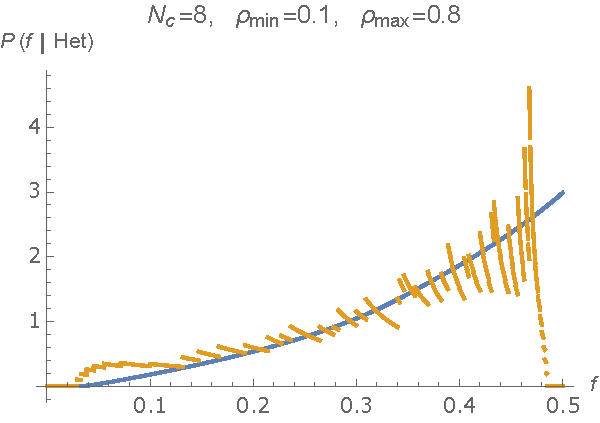
\includegraphics[scale=0.7]{figs/AlleleFractionPrior1.pdf}
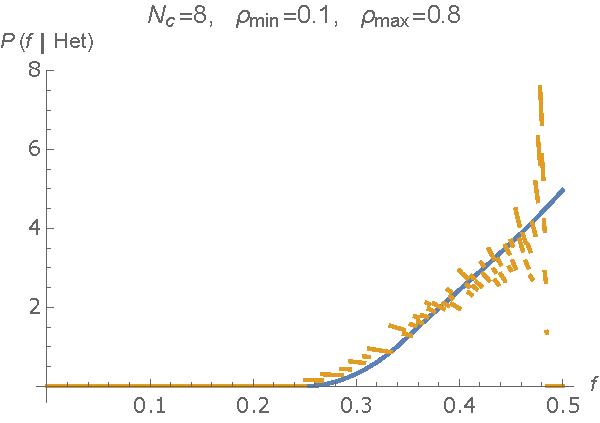
\includegraphics[scale=0.7]{figs/AlleleFractionPrior2.pdf}
\caption{Two examples of the \REF~allele fraction prior $P(f|\mathsf{Het})$ at Het sites based on minimum/maximum non-germline cells and maximum copy number. The blue lines denote the continuous approximation given in Eq.~\eqref{eq:AFpriorcont}, The discontinuous organge lines denote the result with discrete copy number summation given in Eq.~ (the delta function peak at $f=1/2$ is not shown).}
\label{fig:AFprior}
\end{figure}

\noindent {\bf The Bayesian decision rule:} Using the Bayes' theorem, the log odds of heterozygosity is found as:
\begin{equation}
\log \mathrm{odds}(\mathsf{Het}_j) = \log\,P(\{R_{kj}\}|\mathsf{Het}_j) + \log\,P(\mathsf{Het}_j) - \log\,P(\{R_{kj}\}|\mathsf{Hom}_j) - \log\,P(\mathsf{Hom}_j).
\end{equation}
In order to evaluate the right hand side, we need to have knowledge of the prior $P(\mathsf{Het}_j)$. This can be worked out from population statistics. Otherwise, we may use the flat prior $P(\mathsf{Het}_j) = 1/2$.\\


Having the log odds, the decision rule is simple: we call a \HET~site if its odds exceeds a given threshold:
\begin{equation}
\mathrm{Call}~\mathsf{Het}_j \quad \Leftrightarrow \quad \log \mathrm{odds}(\mathsf{Het}_j) > \log\frac{1 - 10^{-s_\mathsf{Het}}}{10^{-s_\mathsf{Het}}} = \log(10^{s_\mathsf{Het}}-1),
\end{equation}
where we have defined the {\em \HET~calling stringency parameter $s_\mathsf{Het}$} as a convenient parametrization of the decision boundary. Finally, we note that the log likelihoods scale linearly with the read depth $N_j$ (each read results in an additional multiplicative term). Therefore, the statistic $\log \mathrm{odds}(\mathsf{Het}_j)$ linearly deviates from the decision threshold $\log(10^{s_\mathsf{Het}}-1) \propto s_\mathsf{Het}$ as the read depth increases.\\

\noindent {\bf Increasing power using haplotype information:}
Todo. The basic idea is to utilize SNP correlations to test multiple correlated sites simultaneously for heterozygosity (1) to increase power, and (2) to improve the prior on $\mathsf{Ref}_j/\mathsf{Alt}_j$. A good starting point to run $\mathsf{HaplotypeCaller}$ on a few normal/tumor reads and check the strength/range/size of correlations between SNP constellations.

\section{GATK CNV/ACNV Models} \label{models}

\subsection{Copy-ratio model} \label{copy-ratio-model}

\SL{SL will fill this in.}

\subsection{Allelic model} \label{allelic-model}
We want a generative model for allelic fractions that infers its parameters from the data.  We observe alt and ref read counts for each het site and wish to infer the minor allelic fraction of every segment.  Let's consider what other hidden variables belong in the model.  Read counts obey an overdispersed binomial distribution in which the probability of an alt read is a site-dependent random variable.  Letting $\theta_j$ be the probability that a mapped read at het $j$ is an alt we have
%
\begin{equation}
P(a_j, r_j | \theta_j) =  \binom{a_j + r_j}{a_j} \theta_j^{a_j} (1-\theta_j)^{r_j} = \binom{n_j}{a_j} \theta_j^{a_j} (1-\theta_j)^{r_j},
\end{equation}
where $a_j$ and $r_j$ are alt and ref read counts and $n_j = a_j + r_j$ is the total read count at site $j$.  Now we consider $\theta_j$.  Suppose site $j$ belongs to a segment with minor allelic fraction $f$ and is alt minor, such that $P({\rm alt}) = f$ and $P({\rm ref}) = 1 - f$ are the probabilities that a random DNA fragment will contain the alt and ref alleles.  Let $x^{\rm alt (ref)}_j = P({\rm mapped} | {\rm alt (ref)})$ be the probabilities that an alt (ref) DNA fragment at site $j$ eventually gets sequenced and mapped.  Then $\theta_j$ is the conditional probability that a mapped read comes from an alt fragment:
%
\begin{align}
\theta_j  &= P( {\rm alt} | {\rm mapped} ) = \frac { P( {\rm alt} ) P( {\rm mapped} | {\rm alt} ) } { P( {\rm alt} ) P( {\rm mapped} | {\rm alt} ) + P( {\rm ref} ) P( {\rm mapped} | {\rm ref} ) } \\
 &= \frac{f x^{\rm alt}_j }{fx^{\rm alt} + (1-f) x^{\rm ref}_j } = \frac{f}{f + (1-f) \lambda_j},
\end{align}
%
where $\lambda_j = x^{\rm ref}_j / x^{\rm alt}_j$ is the ``bias ratio'' of ref to alt sequenceability and mappability at site $j$.  A similar result for ref minor sites follows from substituting $f \leftrightarrow 1 - f$.  In addition to the bias ratio $\lambda_j$ we need an indicator variables $z_j$ with three states, alt minor, ref minor, and an outlier state that gives robustness to anomalous events.  For this outlier state we average the binomial likelihood over all $\theta$ to get:
%
\begin{align}
P(a_j, r_j | {\rm outlier}) = \binom{n_j}{a_j} \int_0^1 \theta_j^{a_j} (1-\theta_j)^{r_j} \, d \theta_j 
= \binom{n_j}{a_j} \frac{a_j! r_j!}{(n_j + 1)!}
\end{align}
%
For notational convenience we give $z_j$ a one-of-$K$ encoding $z_j = (z_{ja}, z_{jr}, z_{jo})$ in which one component equals $1$ and the rest $0$.

The contribution of site $j$ to the likelihood is
%
\begin{equation}
P(a_j, r_j | f_j, \lambda_j, z_j) =  \binom{n_j}{a_j}  
\left[ \frac{f_j^{a_j} (1 - f_j)^{r_j} \lambda_j^{r_j}}{ \left( f_j + (1-f_j) \lambda_j \right)^{n_j}} \right]^{z_{ja}}   
\left[ \frac{(1-f_j)^{a_j} f_j^{r_j} \lambda_j^{r_j}}{ \left( 1 - f_j + f_j \lambda_j \right)^{n_j}} \right]^{z_{jr}}   
\left[ \frac{a_j! r_j!}{(n_j + 1)!} \right]^{z_{jo}}
\label{likelihood}
\end{equation}
%
where $f_s$ is the minor allele fraction of the segment containing site $j$.  We will consider $f$ to be drawn from a uniform distribution on $[0, 1/2]$ -- that is, we give it a flat prior -- but in the future we can obtain some sort of clustering behavior, representing the fact that events in the same subclone that exhibit the same integer copy numbers will have the same minor allelic fractions, by drawing $f_s$ from a Dirichlet process.

We assume that the bias ratios come from a common Gamma distribution with parameters $\alpha, \beta$:
%
\begin{equation}
P(\lambda_j | \alpha, \beta) = \frac{\beta^\alpha}{\Gamma(\alpha)} \lambda_j^{\alpha-1} e^{-\beta \lambda_j}
\end{equation}
%
Note that bias ratios tend to be near $1.0$ and so the choice of distribution is not too important as long as it has adjustable mean and standard deviation.  We choose the Gamma distribution because it is the simplest such distribution on $\mathbb{R}^+$.  We will give the parameters $\alpha$ and $\beta$ a flat prior $P(\alpha, \beta) \propto 1$.

Finally, the indicator $z_j$ is a multinomial random variable distributed according to parameter vector ${\bf \pi}$:
%
\begin{equation}
P(z_{ja(r,o)} = 1 | {\bf \pi}) = \pi_{a(r,o)}
\end{equation}
We set the alt and ref minor probabilities equal so that the only free parameter is $\pi = \pi_o$, with $\pi_{a(r)} = (1 - \pi)/2$.
%
The Bayesian network corresponding to this model is shown in Figure \ref{graphical_model}.
\begin{figure}
$
\begin{array}{c}
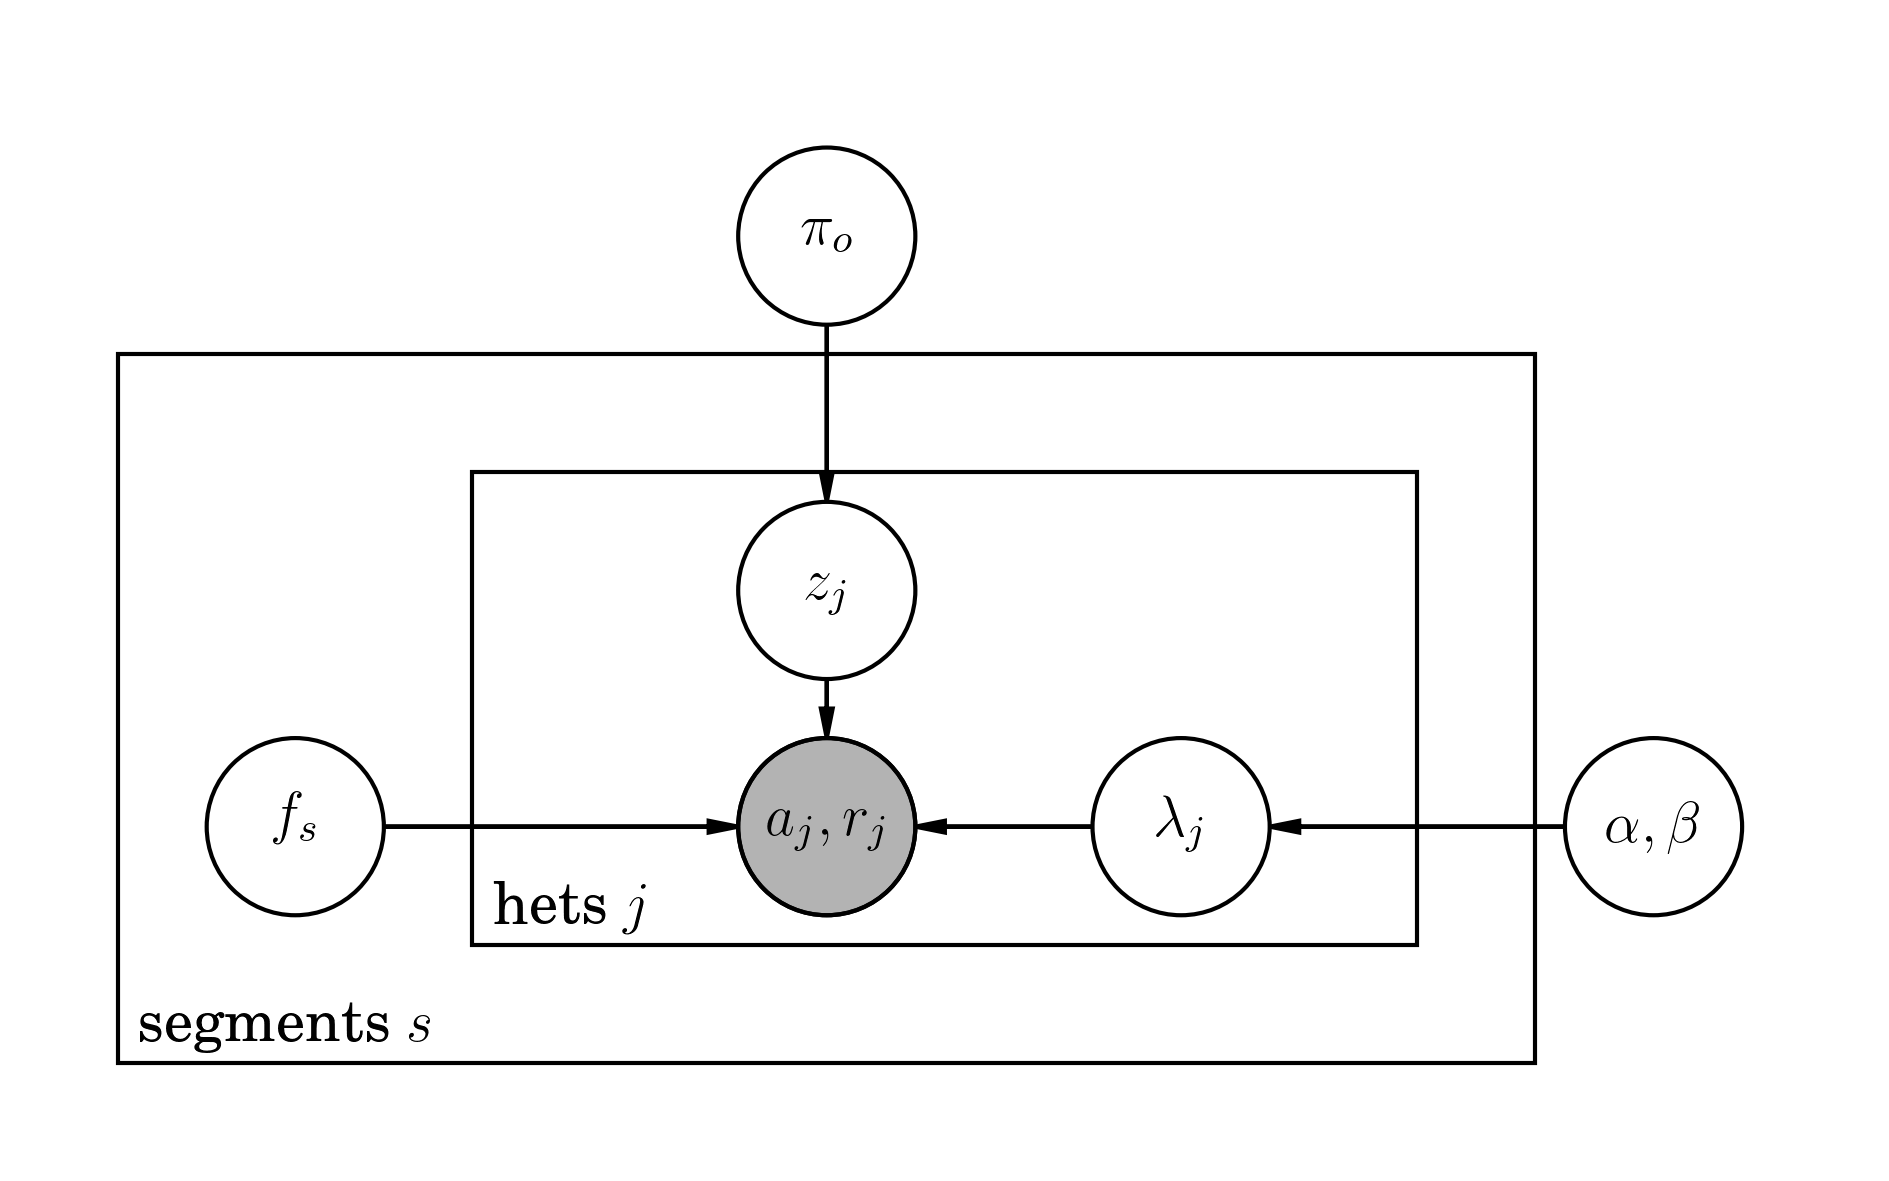
\includegraphics[width=0.8\linewidth]{ACNV_model.png} 
\end{array}
$
\label{graphical_model}
\caption{Graphical model for ACNV allelic model} 
\end{figure}

As with the other parameters, we put a flat prior on ${\rm \pi}$.  Putting all the pieces together the likelihood is
\begin{equation}
\mathbb{L} =\prod_j \frac{\beta^\alpha}{\Gamma(\alpha)} \lambda_j^{\alpha - 1} e^{-\beta \lambda_j}
\left[ \frac{(1-\pi) f_j^{a_j} (1 - f_j)^{r_j} \lambda_j^{r_j}}{ \left( f_j + (1-f_j) \lambda_j \right)^{n_j}} \right]^{z_{ja}}   
\left[ \frac{(1-\pi) (1-f_j)^{a_j} f_j^{r_j} \lambda_j^{r_j}}{ \left( 1 - f_j + f_j \lambda_j \right)^{n_j}} \right]^{z_{jr}}   
\left[ \frac{2 \pi a_j! r_j!}{(n_j + 1)!} \right]^{z_{jo}}.
\label{ACNVlikelihood}
\end{equation}
%
The dependence on $\lambda$ for alt minor sites is
%
\begin{equation}
g(\lambda_j, \alpha, \beta, f_j, a_j, r_j) = \frac{\beta^\alpha}{\Gamma(\alpha)}  \frac{ f_j^{a_j} (1 - f_j)^{r_j}  \lambda_j^{\alpha + r_j - 1} e^{-\beta \lambda_j}}{ \left( f_j + (1-f_j) \lambda_j \right)^{n_j}}.
\end{equation}
For ref minor sites the dependence is the same but with $f \leftrightarrow 1 - f$.  We show in show in Appendix \ref{marginalizing} that this function can be integrated analytically, and thus we can marginalize $\lambda$ out of the model to obtain the likelihood
%
\begin{equation}
\prod_j 
\left[ \frac{1-\pi}{2} \phi(\alpha, \beta, f_j, a_j, r_j)  \right]^{z_{ja}}   
\left[ \frac{1-\pi}{2} \phi(\alpha, \beta, 1 - f_j, a_j, r_j)  \right]^{z_{jr}}   
\left[ \frac{ \pi a_j! r_j!}{(n_j + 1)!}  \right]^{z_{jo}},
\label{marginalized}
\end{equation}
%
where $\phi(\alpha, \beta, f_j, a_j, r_j) = \int_0^\infty g(\lambda, \alpha, \beta, f, a, r) \, d \lambda_j$.  Pseudocode for computing $\phi$ is presented in Appendix \ref{marginalizing}.  Furthermore, marginalizing out $z$ is trivial -- simply sum each term over its three possible states.  We then have a collapsed likelihood
%
\begin{equation}
p(f,\alpha, \beta, \pi) \propto \prod_j 
\left[    \frac{1-\pi}{2} \phi(\alpha, \beta, f_j, a_j, r_j)  +
\frac{1-\pi}{2} \phi(\alpha, \beta, 1 - f_j, a_j, r_j)  +
 \frac{ \pi a_j! r_j!}{(n_j + 1)!}    \right]
 \label{collapsed}
\end{equation}
%
Integrating out the latent variables removes the strongest correlations from the model -- intuitively, $f$ should not be too sensitive to $\alpha$ and $\beta$, for example -- and significantly improves mixing.  The exception is $\alpha$ and $\beta$, since adjusting one with the other fixed changes the mean of the prior on $\lambda$.  Thus we reparameterize in terms of $\mu$ and $\sigma^2$, the mean and variance of the common gamma distribution of biases, where $\alpha = \mu^2 / \sigma^2$ and $\beta = \mu / \sigma^2$.  Due to the weak correlations our MCMC method does not need to be very sophisticated.  We choose to sample each variable with one-dimensional adaptive Metropolis, tuning the proposal step size to achieve some reasonable acceptance rate like $0.4$ or so.  Thus we have completely specified an MCMC scheme for this model, given by Algorithm \ref{ACNV_MCMC}:

\begin{algorithm}
\begin{algorithmic}[1]
\State Initialize all parameters to a maximum likelihood initial guess (see below).
\Repeat
	\State Sample each $f_s$ with adaptive Metropolis
	\State Sample $\pi$ with adaptive Metropolis
	\State Sample $\mu$ with adaptive Metropolis
	\State Sample $\beta$ with adaptive Metropolis
\Until{convergence}
\end{algorithmic}
\caption{MCMC algorithm for ACNV allelic model}
\label{ACNV_MCMC}
\end{algorithm}

We initialize the model by finding the mode of likelihood.  This significantly reduces burn-in time of our MCMC sampling.  Also, it allows us to give the adaptive Metropolis samplers better initial guesses for their step sizes.  Since in practice there is a single global maximum of the likelihood it is easy to find.  After initializing the initialization with rough guesses for the parameters, we successively find one-dimensional maxima adjusting one parameter at a time until the likelihood converges.  One could use multidimensional optimization to obtain faster convergence, but after marginalizing out latent parameters the remaining correlations are weak and thus this simple approach performs quite well.  Since we may delegate one-dimensional maximization to mathematical libraries, the only thing left to describe is our initial coarse guess.

In the initial guess we set the outlier probability $\pi_o = 0.01$, $\mu = 1.0$, and $\sigma^2 = 0.1$.  With the exception of $\sigma^2$ these are all reasonable guesses.  We choose $\sigma^2$ to be larger than what we actually believe because $\mu$ converges more slowly from a bad initial guess if $\sigma^2$ is too small.  The only non-trivial part of the initial guess is the minor allele fractions.  For each segment, we wish to set the minor allele fraction to the number of reads from minor alleles divided by to total number of reads -- this is an unbiased estimator if allelic bias is absent.  The problem is that we have counts of alt and ref reads, not minor and major reads.  Our solution is to weight the alt and ref read counts on each het by probabilities that the het is alt and ref minor, respectively.  That is, we set
%
\begin{equation}
f_S \approx \frac{ \sum_{j \in S} a_j P(z_{ja} = 1) + r_j  P(z_{jr} = 1) }{ \sum_{j \in S} (a_j + r_j) (P(z_{ja} = 1) +  P(z_{jr}=1))}
\end{equation}
%
For this coarse guess we ignore the possibility of outliers, so that $P(z_{ja} = 1) +  P(z_{jr}=1) = 1$.  Ignoring bias and outliers the alt minor likelihood of het $j$ is proportional to $f_j^{a_j} (1-f_j)^{r_j}$.  Since we don't know $f$ yet, we integrate this (including the normalization) from $f=0$ to $f=1/2$ in order to get $P(z_{ja} = 1)$.  This quantity is called the incomplete regularized beta function $I$.  Thus we have
%
\begin{equation}
P(z_{ja} = 1) \approx I(1/2, a_j + 1, r_j + 1), \quad P(z_{jr} = 1) = 1 - P(z_{ja} = 1).
\end{equation}


\subsection{Calling segments after allelic CNV workflow} \label{ACNV-caller}
After running the allelic fraction and copy ratio model, we have a list of segments $s$, each with its own posterior pdfs $f_s^{\rm CR}$ and $f_s^{\rm MAF}$ of the copy ratio and minor allele fraction\footnote{ACNV obtains MCMC samples from these posteriors; we assume that a reasonable distribution has been fit to these posterior samples.}.  That is, $f_s^{MAF}(x)$ is the posterior probability density from ACNV that segment $s$ has minor allele fraction $x$.  We assume that for each segment some fraction $\rho$ of sequenced cells carry $m$ and $n$ copies of the original homologs, while the remaining $1 - \rho$ cells are diploid.  This assumption is compatible with both normal contamination and tumor heterogeneity but not with distinct subclones containing different CNVs at overlapping segments.  It \textit{can} express distinct subclones that inherit a CNV from a common ancestor, as well as a single subclone that incurs overlapping CNVs as long as both are fixed (in the population genetics sense) in that subclone.

Each distinct value of $\rho$ therefore corresponds to a node in the tumor's phylogenetic tree, its value being the proportion of sequenced cells belonging to subclones descended from that node.  We therefore expect its values to be drawn from a discrete multinomial distribution, on which we place a symmetric and sparse Dirichlet prior.  That is, let $\rho$ take on values $\rho_1, \rho_2 \ldots \rho_K$ and let $z_s$ be a binary-valued indicator vector such that $z_{sk} = 1$ if the CNV on segment $s$ occurs in fraction $\rho_k$ of sequenced cells.  Then
\begin{align} 
P(\pi | \alpha) =& \frac{ \Gamma(\alpha) }{\Gamma(\alpha/K)^K} \prod_k \pi_k^{\alpha/K - 1} \\
P(z_s | \pi) =& \prod_k \pi_k^{z_{sk}}
\end{align}
Here $\alpha$ is the concentration parameter such that the smallness of $\alpha / K$ enforces sparseness\footnote{If $\alpha < K$ the prior is singular as $\pi_k \rightarrow 0$ for any $k$.}, i.e. most cluster components will not be used.  The $K \rightarrow \infty$ limit is a Dirichlet process and for finite $K$ to work well, $K$ must be larger than the number of components needed; in practice making $K$ twice as large as the number of components works well.  The expected number of clusters found in data of size $N$ (here, the number of segments) is roughly $\alpha \ln N$, so we place a vague prior on $\alpha$ that corresponds to roughly a single- or double-digit number of clusters.  For example, a broad gamma prior with mean $1$:
%
\begin{equation}
P(\alpha) = {\rm Gamma}(\alpha | 1,1)
\end{equation}
%
We have little prior knowledge on tumor's phylogeny, so we put a uniform prior on the values of $\rho$: $P(\rho_k) = 1$.

Next we relate copy ratio and minor allele fraction to $(m, n, \rho)$.  The total copy number is a weighted sum of $(1-\rho)$ diploid cells and $\rho$ cells with copy number $m+n$.  
%
\begin{equation}
{\rm cr}(m, p, \rho) \equiv \left( 2(1-\rho) + \rho(m + n) \right)/2.
\end{equation}
%
Similarly, the minor allele fraction is a weighted sum of $1 - \rho$ diploid cells with a single copy of the minor allele and $\rho$ cells with ${\rm min}(m,n)$ copies, divided by the total:
%
\begin{equation}
{\rm maf}(m, n, \rho) \equiv \frac{(1- \rho) + \rho ~ {\rm min}(m,n)}{2(1-\rho) + \rho (m + n)}
\end{equation}
%
It is convenient to represent the latent state $(m,n)$ via binary indicator variables $v$ and $w$ with e.g. $v_{sm} = 1, w_{sn} = 1$ if segment $s$ has $m$ and $n$ copies of the original homologs.

Finally, we place a simple factorized multinomial prior on $(m,n)$: $P(m,n) = P(m)P(n) = \phi_m \phi_n$, which we can do if we set of maximum copy number of, say, $m, n < 4$.  The factorization assumption realistic regarding the origin of CNVs but not necessarily regarding their \textit{viability}.  For example, a homozygous deletion could be lethal when a heterozygous deletion is not.  However, we expect this effect to be less dramatic for small segments, which have less phenotypic impact.  Large segments ought to have sufficient statistical power that the prior is less important.  Taking into account the copy ratio and minor allele fraction posteriors from ACNV as well as the mulitnomial prior, the model likelihood is
%
\begin{equation}
P(z_s, v_s, w_s, \pi, \phi, \rho, \alpha) = P(\alpha) \frac{ \Gamma(\alpha) }{\Gamma(\alpha/K)^K} \prod_k \pi_k^{\alpha/K - 1} \prod_{s, k,n,m} \left[ \pi_k \phi_m \phi_n f_s^{\rm CR}({\rm cr}(m,n,\rho_k) f_s^{\rm MAF}({\rm maf}(m,n,\rho_k) \right]^{z_{sk} v_{sm} w_{sn}}
\end{equation}
%

Note that we have simply multiplied of contributions of copy number and minor allele fraction.  This is justified because we inferred the former only from total read counts, while the inference for the latter was \textit{conditioned} on the total read depth of each het.  Thus there is no double-counting of evidence.  This argument is somewhat heuristic because ACNV infers copy number from \textit{target} read counts and minor allele fraction from \textit{SNP} allele counts, but is valid to the extent that total depth at het sites is correlated with depth and the targets they belong to.  For off-target SNPs it is not heuristic at all.

The graphical model is shown in Figure \ref{acnv_caller_fig}.

\begin{figure}
$
\begin{array}{c}
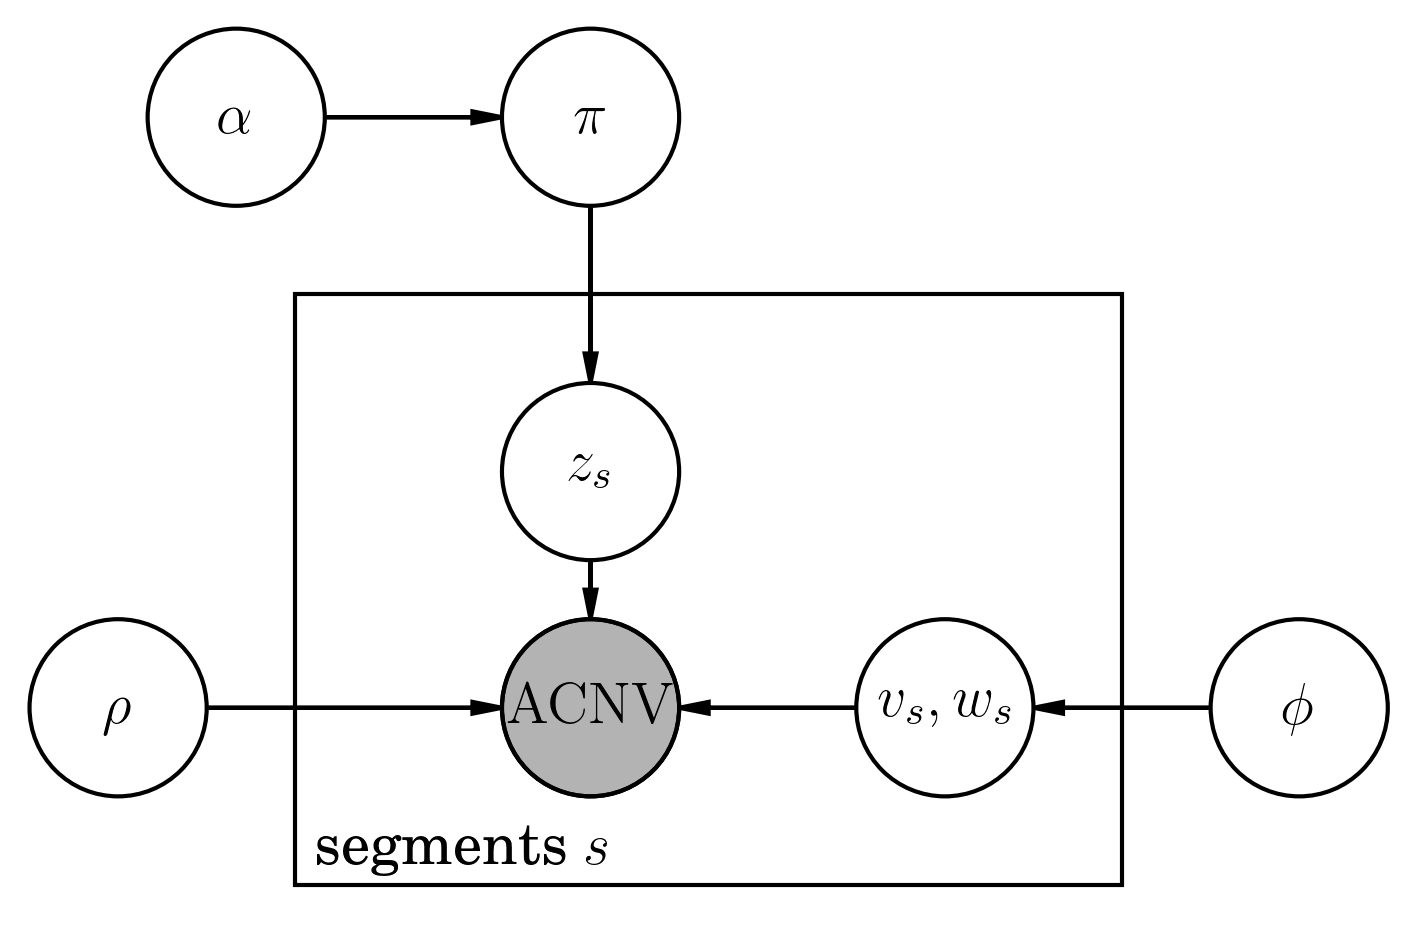
\includegraphics[width=0.8\linewidth]{ACNV_caller_model.png} 
\end{array}
$
\label{acnv_caller_fig}
\caption{Graphical model for ACNV caller.  ``ACNV" represents posterior probability output of ACNV; $v,w$ are indicators of homolog integer copy numbers; $\rho$ is the set of values of ${\rm purity} \times {\rm cancer~cell~fraction}$; $z$ is the corresponding indicator; $\phi$ is the multinomial prior on homolog counts; $\pi$ is the multinomial prior on $z$; $\alpha$ is a Dirichlet concentration parameter encouraging a sparse set of $\rho$ values.} 
\end{figure}

We will obtain maximum likelihood estimates of $\rho$ and $\phi$ and give the remaining variables the variational factorized distribution $p(\alpha, \pi, z, v, w) \rightarrow q(\alpha) q(\pi) q(z,v,w)$. We now proceed to carry out the standard recipe of the EM and variational Bayes algorithms.  Denoting one variable or group of variables by $X$, all other variables by $Z$, and the joint probability by $p(X,Z)$, the mean-field posterior on $X$ is
%
\begin{equation}
\ln q(X) = E_{q(Z)}[\ln p(X,Z)] + {\rm const}
\end{equation}
%
For those variables $X$ for which we seek a point estimate and not a full posterior we employ a similar formula
%
\begin{equation}
X = {\rm arg~max} \left[ E_{q(Z)}[\ln p(X,Z)] \right]
\end{equation}
%

We will henceforth drop the subscript $q(Z)$ from the expectation $E_{q(Z)}$ -- all expectations are with respect to the factorized distribution.  Following this prescription, we find that the posterior on $\alpha$ is
%
\begin{equation}
q(\alpha) \propto \frac{P(\alpha) \Gamma(\alpha)}{\Gamma(\alpha/K)^K} \exp \left(  \frac{\alpha}{K} \sum_k E \left[ \ln \pi_k \right] \right)
\label{q_alpha}
\end{equation}
%
The posteriors on $\pi$ and $\phi$ are
%
\begin{equation}
q(\pi) \propto \prod_k \pi_k^{E [\alpha]/K - 1 + \sum_s E \left[ z_{sk} \right]}, \, q(\phi) \propto \prod_j \phi_j^{\sum_s E \left[ v_{sj} + w_{sj} \right]}
\label{q_pi_phi}
\end{equation}
%
The maximization objective for $\rho$ is
%
\begin{equation}
\rho_k = {\rm arg~max}   \sum_{s, k,n,m} E [z_{sk} v_{sm} w_{sn}] \left[ \ln f_s^{\rm CR}({\rm cr}(m,n,\rho_k) + \ln f_s^{\rm MAF}({\rm maf}(m,n,\rho_k) \right]
\label{M_rho}
\end{equation}
%
Lastly, $q(z,v,w)$ is a categorical distribution which we evaluate by plugging in values:
%
\begin{align}
E \left[z_{sk} v_{sm} w_{sn} \right] = \frac{\phi_m \phi_n e^{E \left[\ln \pi_k \right]} f_s^{\rm CR}({\rm cr}(m,n,\rho_k) f_s^{\rm MAF}({\rm maf}(m,n,\rho_k)}{\sum_{k,m,n} `` \quad  "}
\label{E_z_v_w}
\end{align}
%

Equations \ref{q_alpha} -- \ref{E_z_v_w} require the expectations $E[\alpha]$, $E[\ln \pi]$, $E \left[ z_{sk} \right]$, $E[v_{sj}]$, $E[w_{sj}]$, and $E [z_{sk} v_{sm} w_{sn}]$.  The last of these is the E step Equation \ref{E_z_v_w}.  Three more follow directly from marginalization:
%
\begin{equation}
E \left[ z_{sk} \right] = \sum_{m,n} E [z_{sk} v_{sm} w_{sn}], \, E[v_{sj}] = E[w_{sj}] = \sum_{k, n} E [z_{sk} v_{sj} w_{sn}]
\label{marginals}
\end{equation}
%
By inspection, the Dirichlet posterior $q(\pi)$ of Equation \ref{q_pi_phi} yields the following logarithmic moments:
%
\begin{equation}
E [ \ln \pi_k ] = \psi \left( E [\alpha]/K  + \sum_s E \left[ z_{sk} \right] \right) - \psi \left(  E [\alpha]  + \sum_{s,k} E \left[ z_{sk} \right] \right),
\label{E_pi}
\end{equation}
%
where $\psi$ is the digamma function.  Likewise, $q(\phi)$ is Dirichlet and is maximized with
%
\begin{equation}
\phi_j = \frac{ \sum_s E \left[ v_{sj} + w_{sj} \right] }{ \sum_{s,i} E \left[ v_{si} + w_{si} \right] }
\label{M_phi}
\end{equation}
%
$E[\alpha]$ is not analytic but requires only a single numerical integral per iteration:
%
\begin{equation}
E[\alpha] = \frac{ \int \alpha ~ q(\alpha) ~ d \alpha}{ \int q(\alpha) ~ d \alpha}
\label{E_alpha}
\end{equation}
%

We therefore have a self-contained iteration scheme in terms of expectations only, Algorithm \ref{caller}.

 \begin{algorithm}
\begin{algorithmic}[1]
\State Initialize $E[\alpha] = 1$
\State Initialize $(\rho_1, \rho_2, \ldots \rho_K) = (1/K, 2/K, \ldots 1)$
\State Initialize $E[\ln \pi_j] = \ln (1/K)$ for all $j$.
\State Initialize $\phi$ in some reasonable way, i.e. $\phi_1 > \phi_2 > \phi_0 > \phi_3$.
\Repeat
	\State Update $E [z_{sk} v_{sm} w_{sn}]$ via Equation \ref{E_z_v_w}.
	\State Update $E \left[ z_{sk} \right]$, $E[v_{sj}]$, $E[w_{sj}]$ via Equation \ref{marginals}. 
	\State Update $E [ \ln \pi_k ] $ via Equation \ref{E_pi}
	\State Update $\phi$ via Equation \ref{M_phi}
	\State Update $E [ \alpha ] $ via Equation \ref{E_alpha}
	\State Update $\rho$ via Equation \ref{M_rho}
\Until{convergence}
\end{algorithmic}
\caption{calling allele counts of ACNV segments}
\label{caller}
\end{algorithm}

  Once this converges, the main objects of interest are the posterior probabilities of different allele counts, $P(v_{sm} = 1, w_{sn} = 1) = \sum_k E \left[ z_{sk} v_{sm} w_{sp} \right]$.  For the purposes of guessing phylogeny the fractions $\rho_k$ are also interesting.

\section{Germline Exome CNVs} \label{germline}
The GATK treats germline CNVs differently from somatic CNVs.  This is partly due to fundamental differences, such as the absence of subclones in the germline setting.  However, many arbitrary inconsistencies are historic in nature, arising from the germline algorithm's origins in the XHMM method.  It is important to keep this in mind when reading these notes.  The two most significant differences between the GATK's germline and somatic workflows is are the neglect of allelic information (i.e. alt and ref read counts at het sites) in the germline workflow and the use of an HMM for simultaneous segmentation and calling in the germline workflow.  

We will treat the HMM as a black box.  Although the GATK has its own implementation, the functionality is standard.  Thus we will only describe how we define its states, initial probabilities, transition probabilities, and emission distributions.  Besides that, it suffices to describe what is done to raw coverage data before it is fed into the HMM.

\subsection{Normalization of raw germline data} \label{germline-normalization}
The germline model does not separate the creation of a panel of normals from a case workflow.  Rather, it calls CNVs simultaneously for all samples in a cohort.  Its starting point is an $S \times T$ matrix of raw coverage, where $S$ is the number of samples and $T$ is the number of targets.  We then normalize by each sample's average coverage to get an $S \times T$ \textit{proportional coverage} matrix $P$:
%
\begin{equation}
P_{st} = \frac{ \left( {\rm raw~coverage} \right)_{st} } { {\rm average~depth~of~sample~}s}
\end{equation}
%
Next, as in the somatic workflow, we perform principal components analysis (PCA) on the proportional coverage in order to remove noise due to laboratory conditions etc. from the coverage, leaving (we hope) only a CNV signal and a small amount of residual noise.  For purely historical reasons PCA is expressed here in slightly different terms from the somatic case.  PCA yields a length-$T$ mean proportional coverage vector $\mu$ and set of $M$ principal vectors ${\bf v}_k$, also of length $T$, such that the proportional coverage of each sample is approximated by the mean coverage $\mu$ plus a linear combination of the principal components:
%
\begin{equation}
P_s \approx \mu + \sum_{k=1}^M \beta_{sk} {\bf v}_k
\end{equation}
%
Because the principal components capture the shared variation among all samples, we expect them \textit{not} to capture individual variation due to CNVs.  There is necessarily some contamination because the samples we call are the same samples used to decide the principal components -- there is no separate PoN.  Nonetheless, this effect should be small if there are enough samples.  Therefore, the next step is to produce the tangent-normalized coverage $X$, which is again an $S \times T$ matrix:
%
\begin{equation}
X_s = P_s - \mu -  \sum_{k=1}^M \beta_{sk} {\bf v}_k.
\end{equation}
%
(Here a single subscript for a matrix denotes an entire row).

Finally, the tangent-normalized coverage is converted to a Z-score coverage in which each target is mean-centered (tangent-normalization should yield a mean of zero for each target over all samples, so this part is trivial) and divided by the standard deviation of tangent-normalized coverage of that target over all samples:
%
\begin{equation}
Z_{st} = X_{st} / {\rm std}(X_{\cdot t})
\end{equation}
%

The codebase also allows for filtering at each stage of coverage based on target GC and repeat fraction and various coverage descriptive statistics such as mean, standard deviation and interquartile range of targets across samples and vice versa.  However, we do not yet have a sense of best practices for these.  Furthermore, what constitutes best practices will change as we improve the model.

\subsection{Germline HMM} \label{germline-hmm}
Each sample's Z-score coverage is segmented and called separately via the Viterbi algorithm, which finds the maximum-likelihood solution of an HMM.  The hidden states are neutral, deletion, and duplication -- the XHMM model does not take into account homozygous deletions or multiple duplications.  

The HMM's transition matrix is guided by the principle (an approximation, of course) that there is some underlying biological HMM on a \textit{per-base} level and that \textit{per-target} transitions are simply the realization of this underlying HMM on a coarser scale.  The per-base transition matrix is defined by two parameters.  The first is the probability $p$ to to make a transition from a neutral state to a CNV state.  Equivalently, $1/p$ is, roughly, the average separation between CNVs.  The second is the probability $1/D$ that a CNV state ends.  Equivalently, $D$ is the average CNV length in base pairs.   The probability for a CNV to terminate between two consecutive targets a distance $d$ apart is $1 - e^{-d/D}$.
  
Letting $f = e^{-1/D}$ the transition matrix $T$ between two adjacent bases is
%
\begin{equation}
T = \bordermatrix{ {\rm from} \backslash {\rm to} & - & 0 & + \cr
      - & f & 1-f & 0 \cr
      0 & p & 1-2p & p \cr
      + & 0 & 1-f & f}
\end{equation}
%
We neglect transitions between different types of CNVs at consecutive bases, which are extremely rare.  Note that this in no way precludes CNVs of different types occurring at adjacent targets.  The transition matrix for two targets separated by $d$ bases is $T^d$.  We can compute this very cheaply by first diagonalizing $T$ as $T = U \Sigma V^T$, where $\Lambda$ is a diagonal matrix.  Then $T^d = U^T \Lambda^d U$.  For numerical stability one usually works with log transition probabilities, so we have:
%
\begin{align}
\log \left(T^d \right)_{ij} =& \log \sum_k U^T_ik \Lambda^d_{kk} U_{kj} \\
				    =& \log \sum_k \Lambda^d_{kk} U_{kj} U_{ki} \\ 
				    =& \log \sum_k \exp \left( d \log \Lambda_{kk} + \log U_{kj} + \log U_{ki}  \right)
\end{align}
%
In this form we can work entirely in log space and exploit the log-sum-exp trick for stability.


The emission model is as follows.  Each hidden state emits a normally-distributed Z-score.  The means are $-M$, 0, and $+M$ for deletion, neutral, and duplication states, respectively, where $M$ is s user-specified parameter whose default is 3.  Each emission distribution is given unit variance.  This model is quite wrong.  Consider a duplication.  The tangent-normalized coverage ought be be roughly 0.5 times the proportional coverage -- the raw coverage is $3/2$ that of a diploid target, leaving $1/2$ remaining after (ideal) tangent-normalization.  Then division by the target standard deviation to get a Z-score yields who-knows-what.  Since different targets have different average proportional coverage, the global parameter $M$ is misguided.  Basically, the current model is not a model at all, but a heuristic.

\section{Proposed Methods} \label{proposed-methods}

\subsection{Using Panel of Normals for Allelic Fraction Model} \label{allelic-PoN}

The GATK ACNV allelic model learns a global distribution on allelic biases and uses it as a shared prior for the allelic biases of SNPs.  While better than nothing, it would be much more powerful to use prior knowledge of the allelic bias at each SNP individually.  We can learn these per-SNP biases from a panel of normals using the allelic model, but with two simplifications.  First, minor allele fractions are always $1/2$ since normal samples are diploid and do not exhibit subclonality.  Second, we do not account for outliers; that is, we set the outlier probability $\pi = 0$.  The reason for this is that the panel of normals reflects typical distributions of allelic biases and censoring data via an outlier classification could render these distributions artificially tight.  If the allelic bias at some SNP site varies a lot we want to know about it. The overall likelihood is
%
\begin{align}
& \prod_j \frac{\beta^\alpha}{\Gamma(\alpha)} \lambda_j^{\alpha - 1} e^{-\beta \lambda_j}
\prod_{s \in \mathcal{H}_j}
 \frac{  \lambda_j^{r_{sj}}}{ \left( 1 + \lambda_j \right)^{n_{sj}}}  \\
 = & \prod_j \frac{\beta^\alpha}{\Gamma(\alpha)} e^{-\beta \lambda_j}
 \frac{  \lambda_j^{\alpha + r_{ \cdot j} - 1}}{ \left( 1 + \lambda_j \right)^{n_{\cdot j}}} 
 \label{ACNVponlikelihood}
\end{align}
%
where $\lambda_j$ is the allelic bias ratio of SNP $j$ (for samples sequenced and mapped using the same technology as the panel of normals), $\mathcal{H}_j$ is the set of samples in the panel of normals that are heterozygous at SNP $j$, $r_{\cdot j} = \sum_{s \in \mathcal{H}_j} r_{sj}$, and $n_{\cdot j} = \sum_{s \in \mathcal{H}_j} n_{sj}$.  As before, the biases are assumed to come from a common distribution ${\rm Gamma}(\alpha, \beta)$, but due to the large number of samples in the panel of normals the data will yield a posterior distribution on each $\lambda_j$ that may be quite different from the global prior.  It is these posteriors that we will use as input to ACNV.  Although they are the object of interest, however, we will first marginalize them out of the likelihood in order to obtain maximum likelihood estimates of $\alpha$ and $\beta$.  We have in fact already performed this marginalization -- Equation \ref{ACNVponlikelihood} is the special case $f = 1/2$, $\pi = 0$ of the allelic-model likelihood, Equation \ref{likelihood}, and thus its marginalization over latent variables is obtained by substituting $f = 1/2$, $\pi = 0$ into Equation \ref{collapsed}, which yields
%
\begin{equation}
p(\alpha, \beta) = \prod_j \phi(\alpha, \beta, f = 1/2, n_{\cdot j} - r_{\cdot j}, r_{\cdot j}).
\end{equation}
%
This likelihood is easily maximized numerically to obtain MLE values of $\alpha$ and $\beta$.  Having done this, we can then approximate the posterior on each $\lambda_j$ as a gamma distribution using the method of Appendix \ref{marginalizing}.  As shown there, the posterior on $\lambda_j$ is ${\rm Gamma}(\rho_j, \tau_j)$ where $\rho_j$ and $\tau_j$ are computed in Algorithm \ref{phi_calculation}, with $a \rightarrow n_{\cdot j} - r_{\cdot j}$ and $r \rightarrow r_{\cdot j}$.

Once we have the posteriors on each $\lambda_j$ from the panel of normals, they are used as priors for $\lambda_j$ in the ACNV allelic model.  This obviates the hyperparameters $\alpha$ and $\beta$, and Equation \ref{collapsed} becomes
%
\begin{equation}
p(f, \pi) \propto \prod_j 
\left[    \frac{1-\pi}{2} \phi(\rho_j, \tau_j, f_j, a_j, r_j)  +
\frac{1-\pi}{2} \phi(\rho_j, \tau_j, 1 - f_j, a_j, r_j)  +
 \frac{ \pi a_j! r_j!}{(n_j + 1)!}    \right]
 \label{collapsed_using_pon}
\end{equation}
%
where $f$ and $\pi$ may once again be sampled via adaptive Metropolis.

\subsection{Generative Model for Read Counts} \label{coverage-model}

\noindent We wish to address several goals in this section:

\begin{enumerate}

\item Connect copy ratio (or copy number) and raw read counts in a single probabilistic model without transforming the data.

\item Take into account the Poisson nature of coverage depth, thereby giving less weight to low-coverage targets and separating the inherent variance due to Poisson statistics from experimental noise.  We want to use the panel of normals to subtract only the latter.

\item Choose the number of principal components to use in an automatic and principled manner.

\item Use an algorithm that does not waste time calculating all principal components when we only want the few most significant ones.

\item Make a universal panel of normals for both sexes by taking into account targets on sex chromosomes on par with autosomal targets.

\item A reliable method for detecting and excluding outlier samples from the panel of normals, in particular, those with abnormal ploidy.

\item Correct for CNV events that occur in the panel of normals.

\end{enumerate}

Suppose we have vectors of read counts over a set of $T$ targets for $S$ samples, $\vn_s, \, s = 1 \ldots S$ where $n_{st}$ is the coverage of sample $s$ at target $t$. In order to include both sexes on an equal footing, we further define a ``ploidy matrix'' $\PP_{st}$ such that $\PP_{st}$ is the ploidy\footnote{For human autosomal targets, $\PP_{st} = 2$ for both sexes. In female samples, $P_{st} = 2$ for X chromosome targets and $P_{st} = 0$ for Y chromosome targets. Finally, $P_{st} = 1$ for X and Y chromosomes in male samples} of target $t$ of sample $s$. We imagine that laboratory conditions for a particular sample yielding an underlying bias vector $\vb_s$, where $e^{b_{st}}$ is the propensity of target $t$ to be captured, sequenced, and mapped in the preparation of sample $s$.  Suppose also that sample $s$ has an average depth $d_s$ and a vector of copy numbers $\vc_s$, where the latent variable $c_{st}$ is the copy number of sample $s$ at target $t$.  Our model for coverage is\footnote{In Equation \ref{coverage_model} the quantity $d_s$ is a hypothetical quantity representing average coverage in the absence of bias.  Since this is impossible to know we use average coverage instead.  This doesn't matter since any constant factor will be absorbed into $e^b$ via the parameter $\vm$.}:
%
\begin{equation}
n_{st} \sim {\rm Poisson}(d_s \PP_{st} c_{st} e^{b_{st}})
\label{coverage_model}
\end{equation}
%
We can achieve many of the goals listed above by performing probabilistic PCA not on $\vn$ directly but rather on $\vb$.  This is one reason why we choose a Poisson parameter proportional to $e^b$ and not simply $b$ -- probabilistic PCA involves a normal distribution on $\vb_s$, whereas the Poisson parameter must be positive.  Furthermore, since PCA is a linear model with additive effects of different latent features, using $e^b$ represents multiplicative effects, which is more plausible.  Our model is
%
\begin{align}
\vz &\sim \norm(\vzero, \vI), \nonumber\\
\vb &\sim \norm(\vW \vz + \vm, \vPsi),
\end{align}
%
where $\vz \in \mathbb{R}^D$ is a low-dimensional latent vector of laboratory conditions, $\vW \in \mathbb{R}^{T \times D}$ is a linear map from latent space to target space, $\vm \in \mathbb{R}^T$ is the vector of mean biases, and $\vPsi \in \mathbb{R}^{T \times T}$ is a diagonal matrix of residual variance not explained by the latent features. We approximate the Poisson as a Gaussian (an excellent approximation for $n_{st} \gtrsim 1000$) and expand the argument of the Gaussian exponential about the mode of $b_{st}$ to quadratic order to obtain:
%
\begin{equation}
{\rm Poisson}(n_{st} | d_s c_{st} e^{b_{st}}) \approx \norm(b_{st} | m_{st}, \Sigma_{st}),
\end{equation}
where:
\begin{align}
m_{st} &= \ln(n_{st}/(\PP_{st} c_{st} d_s)), \nonumber\\
\Sigma_{st} &= 1/n_{st}.
\end{align}
Note that $\Sigma_{st}$ can be thought of as the width of the distribution of $b_{st}$ about its maximum likelihood estimate such that in the limit $n_{st}, d_s \rightarrow \infty$, ${\rm Poisson}(n_{st} | d_s c_{st} e^{b_{st}}) \rightarrow \delta(b_{st} - b^*_{st})$ where $b^*_{st} = \lim_{n,d \rightarrow \infty} m_{st}$ is the true bias. The above approximation, while being excellent for well-covered targets, inevitably breaks down for targets that are uncovered {\em ex ante} in some samples, such as $Y$ chromosome targets in female samples. To this end, we define a ``sample-target mask matrix'' $\MM_{st}$ such that $\MM_{st} = 0$ if $\PP_{st} = 0$, and $\MM_{st} = 1$ if $\PP_{st} \neq 0$, and for each sample-target pair $(s,t)$, we only consider targets where the $\MM_{st} \neq 0$ in the joint likelihood function. The latter is thus written as:
\begin{equation}
P(\vn, \vb, \vz | \vc, \vW, \vm, \vPsi) = \prod_s \norm(\vz_s | \vzero, \vI) \prod_{t | \MM_{st} \neq 0} \norm(b_{st} | (\vW \vz_s)_t + m_t, \Psi_t) \, \norm(b_{st} | m_{st}, \Sigma_{st})
\end{equation}
We can integrate out $\vb$ via the identity $\int_{-\infty}^{+\infty} \norm(x | \mu_1, \sigma_1^2) \, \norm(x | \mu_2, \sigma_2^2) \, \mathrm{d}x = \norm(\mu_1 | \mu_2, \sigma_1^2 + \sigma_2^2)$ to obtain:
%
\begin{equation}
P(\vn, \vz | \vc, \vW, \vm, \vPsi) = \prod_s \norm(\vz_s | \vzero, \vI) \prod_{t | \MM_{st} \neq 0} \norm(m_{st} | (\vW \vz_s)_t + m_t, \Psi_t + \Sigma_{st})
\label{coverage_likelihood}
\end{equation}
Save for the presence of a sample-dependent bias uncertainy $\Sigma_{st}$, our learning objective is essentially the factor analysis problem. The MLE for parameters $(\vPsi, \vW, \vm)$ can be obtained via the EM algorithm. The presence of $\Sigma_{st}$, in particular its dependence on $s$, introduces undesirable complexities which we wish to avoid. To gain more insight about the role of $\Sigma_{st}$, let us mrginalizing $\vz_s$ from Eq.~\eqref{coverage_likelihood}. The final result can be put in a simple form using Woodbury identity and properties of projection matrices:
%
\begin{equation}
P(\vn | \vc, \vW, \vm, \vPsi) \propto \exp \left( -\frac{1}{2} \sum_s (\vm - \vm_s)^T \vM_s (\vPsi + \vSigma_s + \vM_s \vW \vW^T \vM_s)^{-1} \vM_s (\vm - \vm_s) \right)
\label{marginalized coverage_likelihood}
\end{equation}
%
To simplify the discussion, let us assume that all samples share the same targets, i.e. $\vM_s = \mathbb{I}$.
First, note that $\vPsi + \vW \vW^T$ is the covariance of log-coverage due to experimental conditions, both those included explicitly in $\vW$ and the residual, unexplained covariance $\vPsi$. The quantities $\vPsi + \vSigma_s + \vW \vW^T$ are essentially weighting factors that decrease the role of lower-coverage samples (i.e. those with larger $\vSigma$) in the likelihood. If variations in $\vSigma$ tend to be small compared to $\vPsi + \vW \vW^T$, then these weights will be very similar between samples and we may use the simple formula that assigns each sample the same weight. {\em It is an empirical fact that the noise before normalization is much greater than noise after normalization, which implies that $\vSigma$ is small compared to $\vPsi + \vW \vW^T$. Variations in $\vSigma$ are, of course, even smaller, especially in the typical case that all PoN samples have similar depth.} Furthermore, if the depths of PoN samples are not correlated with their positions in latent space (as is reasonable) our approximation is an unbiased estimator, because for any given position in latent space our failure to use the exact weights will on average wash out.  Finally, suppose, contrary to empirical fact, that $\vSigma$ tended to be large compared to $\vPsi + \vW \vW^T$. In this case, either the shared source of bias is small and we don't need this fancy model in the first place, or the depth of coverage is very poor, in which case accurate normalization is hopeless regardless. In summary, replacing $\Sigma_{st}$ with a typical sample-indendent value $\bar{\vSigma}$ is a very reasonable approxmiation.

A natural choice for $\bar{\Sigma}_t$ will be made apparent soon. In the meantime, we notice that the $\vSigma_s$ always appears in addition to $\vPsi$ such that the specific choice of $\bar{\Sigma}_t$ may seem to be immaterial: if $\vPsi^*$ is the MLE estimate obtained using the choice $\bar{\vSigma}^*$, we may infer that $\vPsi^* + \bar{\vSigma}^* - \bar{\vSigma}'$ is the MLE estimate had we used $\bar{\vSigma}'$ instead. However, the constraint $\Psi_t > 0$ implies that $\Psi^*_t + \bar{\Sigma}_t > 0$, such that our choice of $\bar{\Sigma}_t$ effectively sets a lower bound on the unexplained variance.\\


\noindent {\bf EM algorithm for obtaing MLE of $(\vW, \vPsi, \vm)$:} For fixed $\vc$, we may obtain maximum likelihood estimates of the parameters via an iterative EM approach in which we alternate between computing the Gaussian posteriors of each $\vz_s$ (E step) and maximizing the log-likelihood with respect to $\vW$, $\vSigma$, and $\vm$ (M step). This is similar to the factor analysis model discussed in Chapter 12 of Bishop. We note calling $\vc$ while learning $(\vW, \vPsi, \vm)$ allows us to correct for CNV events that may be present in the panel of normals\footnote{If our copy-ratio calling algorithm is a maximum-likelihood method, for example calling via the Viterbi algorithm for an HMM, then provided that our likelihood is averaged with respect to the E step for $\vz$ the entire process including optimization of $(\vc, \vW, \vPsi, \vm)$ is an EM algorithm and thus will increase likelihood at each iteration and converge.}.\\

The E step follows from substituting $\vPsi \rightarrow \vPsi_s \equiv  \vPsi + \vSigma_s$ in Bishop's Eqs. 12.66-67 and including the sample-target mask matrix $\vM$. The result is:
%j
\begin{align}
\vG_s &= \left( \vI + \vW^T \vM_s \vPsi_s^{-1} \vW \right)^{-1}, \nonumber\\
\EE \left[ \vz_s \right] &= \vG_s \vW^T \vM_s \vPsi_s^{-1} (\vm_s - \vm), \nonumber\\
\EE \left[ \vz_s \vz_s^T \right] &= \vG_s + E[\vz_s] E[\vz_s]^T.
\end{align}
%
In the M step, we calculate the expectation value of the complete-data log likelihood with respect to the posperior estimate of $\vz_s$. Save for a constant, the result is:
%
\begin{equation}
\mathcal{L} = -\frac{1}{2} \sum_{st} \left\{ M_{st} \ln \Psi_{st} + M_{st} \Psi_{st}^{-1} \left[  \left( \vW \EE[\vz_s \vz_s^T] \vW^T \right)_{tt} +2 (m_t - m_{st}) \left( \vW \EE[\vz_s] \right)_t + (m_t - m_{st})^2 \right] \right\},
\end{equation}
%
The stationarity condition for $\mathcal{L}$ with respect to $\vm$ gives: 
\begin{align}
m_t = \left(\sum_s \vM_s \vPsi_{s}^{-1} \right)^{-1} \sum_s \left[ \vM_s \vPsi_{s}^{-1}  (\vm_{s}  - \vW  \EE[\vz_{s}] ) \right].
\end{align}
The stationarity condition with respect to $\Psi_t$ gives:
\begin{equation}\label{eq:psi_stationarity}
\sum_s M_{st}\left[\frac{1}{\Psi_t + \Sigma_{st}} - \frac{B_{st}}{(\Psi_t + \Sigma_{st})^2} \right] = 0,
\end{equation}
where:
\begin{equation}
B_{st} = \left( \vW E[\vz_s \vz_s^T] \vW^T \right)_{tt} +2 (m_t - m_{st}) \left( \vW E[\vz_s] \right)_t + (m_t - m_{st})^2
\end{equation}
The above nonlinear equation must be solved for each target, which is a computationally demanding task for a large number of targets. If this is to be avoided, we offer two approximation schemes:\\

\noindent {\bf (Scheme 1) Assuming small sample to sample variations in $\Sigma_{st}$:} Had $\Sigma_{st}$ been constant, then Eq.~\eqref{eq:psi_stationarity} would have the following simple solution:
\begin{equation}
\Psi^\mathrm{approx}_t = \llangle \mathbf{B} \rrangle_t - \bar{\Sigma}_t,
\end{equation}
where $\bar{\Sigma}_t$ is the sample-independent value of $\Sigma_{st}$, and we have defined the double angle bracket average as:
\begin{equation}\label{eq:psi_approx}
\llangle \mathbf{B} \rrangle_t \equiv \frac{\sum_s M_{st}B_{st}}{\sum_s M_{st}}.
\end{equation}
It is tempting to replace $\bar{\Sigma}_t$ with its $M$-averaged value. However, a more principled approach is to choose $\bar{\Sigma}_t$ such that the approximation solution given in \eqref{eq:psi_approx} is as close to the exact solution as possible. To this end, we assume $\Sigma_{st} = \bar{\Sigma}_t + (\Sigma_{st} - \bar{\Sigma}_t)$ such that $|\Sigma_{st} - \bar{\Sigma}_t| \ll \bar{\Sigma}_t$, expand Eq.~\eqref{eq:psi_stationarity} in $\Sigma_{st} - \bar{\Sigma}_t$ to linear order, and require that $\Psi^\mathrm{approx}_t$ represents the exact solution. This procedure yields:
\begin{equation}
\bar{\Sigma}_t = \frac{2 \llangle \mathbf{B} \vSigma \rrangle_t - \llangle \vSigma \rrangle_t \llangle \mathbf{B}\rrangle_t}{\llangle \mathbf{B}\rrangle_t}.
\end{equation}
Plugging this result back in Eq.~\eqref{eq:psi_approx}, we find:
\begin{equation}
\Psi^\mathrm{approx}_t = \llangle \mathbf{B} \rrangle_t + \llangle \vSigma \rrangle_t - 2 \, \frac{\llangle \mathbf{B} \vSigma \rrangle_t}{\llangle \mathbf{B}\rrangle_t}.
\end{equation}
This solution is accurate to linear order in deviations of $\Sigma_{st}$ about $\bar{\Sigma}_t$.\\

\noindent {\bf (Scheme 2) Newton iterations:} The complexity of solving Eq.~\eqref{eq:psi_stationarity} numerically is not too high given that the Hessian matrix is diagonal. Expanding $\mathcal{L}$ about $\vPsi_0$, we find:
\begin{equation}
\mathcal{L}(\vPsi) = \mathcal{L}(\vPsi_0) + \alpha_t \, (\Psi_t - \Psi_{0,t}) + \frac{1}{2} \, \beta_t \, (\Psi_t - \Psi_{t,0})^2 + \ldots
\end{equation}
where:
\begin{align}
\alpha_t &= \frac{\partial \mathcal{L}}{\partial \Psi_t} = -\frac{1}{2}\sum_s M_{st}\left[\frac{1}{\Psi_t + \Sigma_{st}} - \frac{B_{st}}{(\Psi_t + \Sigma_{st})^2}\right],\nonumber\\
\beta_t &= \frac{\partial^2 \mathcal{L}}{\partial \Psi_t^2} = +\frac{1}{2}\sum_s M_{st}\left[\frac{1}{(\Psi_t + \Sigma_{st})^2} - \frac{2B_{st}}{(\Psi_t + \Sigma_{st})^3}\right].
\end{align}
The Newton's approximate solution is therefore:
\begin{equation}
\Psi_{t,1} = \Psi_{t,0} - \frac{\alpha_t(\vPsi_0)}{\beta_t(\vPsi_0)}.
\end{equation}
One may start iterations using the result of Scheme 1 as the initial guess and continue until convergence.\\

In the M step equation for $\vW$, we incorporate an automatic relevance determination (ARD) prior:
%
\begin{align}
P(\vW) =& \prod_\mu \left( \frac{\alpha_\mu}{2 \pi} \right)^{T/2} \exp \left( -\frac{1}{2} \alpha_\mu \sum_t W_{t\mu}^2  \right).
\end{align}
%
If $\alpha_\mu \rightarrow \infty$, latent feature $\mu$ is effectively turned off. Thus we can initially choose a liberal estimate of $D$ and the model will automatically become more parsimonious. The M step log likelihood times the ARD prior depend on the $t$-th row $\vW_{t \cdot}$ of $\vW$ as:
%
\begin{equation}
 -\frac{1}{2}   \left( -\sum_\mu \ln \alpha_\mu  + \vW_{t \cdot} \left(\vA +  \vQ_t  \right) \vW_{t \cdot}^T - 2 \vW_{t \cdot} \vv_t  \right),
 \label{ARD_likelihood}
\end{equation}
%
where $\vA \equiv {\rm diag}(\alpha_1, \alpha_2 \ldots \alpha_D)$ and we have defined:
%
\begin{equation}
\vQ_t = \sum_s M_{st} \Psi_{st}^{-1} \, \EE\left[\vz_s \vz_s^T\right], \, \qquad \vv_t = \sum_s M_{st} \Psi_{st}^{-1} (m_{st} - m_t)\, \EE[\vz_s].
\end{equation}
%
The maximum a posterior result for $\vW_{t \cdot}$ is:
%
\begin{equation}
\vW_{t \cdot} = \left(  \vA + \vQ_t \right)^{-1} \vv_t
\label{M_step_W}
\end{equation}
%
In the approximation $\vSigma_s \rightarrow \bar{\vSigma}$, this formula is unchanged but $\vQ_t$ is $S$ times as fast to calculate. The other M steps and the E step are not affected by the ARD prior. To determine $\alpha_\mu$, we re-exponentiate Eq.~$\eqref{ARD_likelihood}$\footnote{This is the distribution on $\vW$ that we would obtain from a mean-field variational factorization $q(\vz) q(\vW)$.} and integrate out $\vW$ to obtain the evidence for $\vA$:
%
\begin{align}
P(\vn | \vA) \propto& \prod_k \alpha_k^{T/2} \prod_t \int e^{-\frac{1}{2} \vW_{t \cdot} (\vA + \vQ_t) \vW_{t \cdot}^T - \vW_{t \cdot} \vv_t} \, \mathrm{d} \vW_{t \cdot}
\label{ARD_evidence}
\end{align}
%
The ARD coefficients $\alpha$ are determined by maximizing the log evidence.  That is, we set
\begin{align}
\frac{\partial}{\partial \alpha_k} \ln P(\vn | \vA) = 0 \Rightarrow  \frac{1}{2} \left( \frac{T}{\alpha_\mu}  - \sum_t \ave{W_{t\mu}^2} \right) = 0 \Rightarrow \alpha_\mu = \frac{T}{\sum_t \ave{W_{t\mu}^2}},
\end{align}
where the average $\ave{W_{t\mu}^2}$ is taken with respect to the density $q(\vW_{t \cdot}) \propto e^{-\frac{1}{2} \vW_{t \cdot} (\vA + \vQ_t) \vW_{t \cdot}^T - \vW_{t \cdot} \vv_t}$.  Completing the square, we find that $q(\vW_{t \cdot})$ is Gaussian with covariance $(\vA + \vQ_t)^{-1}$ and mean $(\vA + \vQ_t)^{-1} \vv_t$.  Note that this mean is precisely the M step value for $q(\vW_{t \cdot})$, as we would hope!  Thus we get
%
\begin{equation}
\ave{W_{t\mu}^2} = W_{t\mu}^2 + (\vA + \vQ_t)^{-1}_{\mu\mu}
\end{equation}\\
%

\textcolor{red}{(The summary must be updated) -- } Let us now summarize these steps.  First, in exact mode we have
\begin{itemize}
\item E step: $\vG_s = \left( \vI + \vW^T \vPsi_s^{-1} \vW \right)^{-1}, \,
E \left[ \vz_s \right] = \vG_s \vW^T \vPsi_s^{-1} (\vm_s - \vm), \,
E \left[ \vz_s \vz_s^T \right] = \vG_s + E[\vz_s] E[\vz_s]^T$

$\vG_s$ and all the $E[\vz_s]$ are each $O(D^2 T S)$.  $E[\vz_s \vz_s^T]$ is $O(D^2 S)$.  The E step overall is $O(D^2 T S)$.

\item $\vm = \left( \sum_s \vPsi_{s}^{-1} \right)^{-1} \sum_s \left[ \vPsi_{s}^{-1}  (\vm_{s}  - \vW  E[\vz_{s}] ) \right]$ is $O(D T S)$.

\item  $ \beta_{st} =\left( \vW E[\vz_s \vz_s^T] \vW^T \right)_{tt} +2 (m_t - m_{st}) \left( \vW E[\vz_s] \right)_t + (m_t - m_{st})^2$ is $O(D^2 T S)$

\item Solving $\sum_s \left[ \frac{1}{\Psi_t + \Sigma_{st}} - \frac{\beta_{st}}{(\Psi_t + \Sigma_{st})^2} \right] = 0$ for each $t$ is $O(T S)$ with a prefactor equal to the number of evaluations required to find a root.  As long as this number is less than $D^2$ this step is subleading.

\item $\vQ_t = \sum_s \Psi_{st}^{-1} E[\vz_s \vz_s^T]$ is $O(D^2 T S)$.

\item $\vv_t = \sum_s \Psi_{st}^{-1} (m_{st} - m_t)E[\vz_s ]$ is $O(D T S)$.

\item $ \vW_{t \cdot} = (\vA + \vQ_t)^{-1} \vv_t$ is $O(D^3 T)$.

\item $\ave{W_{t\mu}^2} = W_{t\mu}^2 + (\vA + \vQ_t)^{-1}_{\mu\mu}$ is $O(D^3 T)$.

\item $\alpha_\mu = T / \sum_t \ave{W_{t\mu}^2}$ is $O(D T)$.

\end{itemize}

In approximate mode
\begin{itemize}
\item E step: $\vG = \left( \vI + \vW^T \bar{\vPsi}^{-1} \vW \right)^{-1}, \,
E \left[ \vz_s \right] = \vG \vW^T \bar{\vPsi}^{-1} (\vm_s - \vm), \,
E \left[ \vz_s \vz_s^T \right] = \vG + E[\vz_s] E[\vz_s]^T$

$\vG$ is $O(D^2 T)$.  $E[\vz_s \vz_s^T]$ is $O(D^2 S)$.  $\vG_s \vW^T \vPsi_s^{-1}$, which is common to all $E[\vz_s]$, is $O(D^2 T)$ after which $E[\vz_s]$ is $O(D T S)$.  $E[\vz_s \vz_s^T]$ is $O(D^2 S)$.  The E step overall is $O(D T S)$.

\item $\vm = \frac{1}{S} \sum_s \vm_s$ is a one-time cost of $O(T S)$.

\item $\sum_s \beta_{st} =\left( \vW \left( \sum_s E[\vz_s \vz_s^T] \right) \vW^T \right)_{tt} +2 \left( \vW \left( \sum_s (m_t - m_{st}) E[\vz_s] \right) \right)_t + \sum_s (m_t - m_{st})^2$ is $O(D^2 T)$.

\item Given $\sum_s \beta_{st}$, $\Psi_{tt} = \frac{1}{S} \sum_s \beta_{st} - \bar{\Sigma}_{tt}$ is $O(T)$.

\item $\vQ_t =  \bar{\Psi}_{t}^{-1} \sum_s E[\vz_s \vz_s^T]$ is $O(D^2 (S + T))$.

\item $\vv_t = \sum_s \bar{\Psi}_{t}^{-1} (m_t - m_{st})E[\vz_s ]$ is $O(D T S)$.

\item $ \vW_{t \cdot} = (\vA + \vQ)^{-1} \vv_t$ is $O(D^2 T)$.

\item $\ave{W_{t\mu}^2} = W_{t\mu}^2 + (\vA + \vQ)^{-1}_{\mu\mu}$ is $O(D T)$.

\item $\alpha_\mu = T / \sum_t \ave{W_{t\mu}^2}$ is $O(D T)$.
\end{itemize}

In exact mode the leading cost is a few terms of $O(D^2 T S)$ flops, each with small prefactors, per iteration.  In approximate mode it is $O(D T S)$ flops.  Assuming a total prefactor of $10$ and $T = 2 \times 10^5$, $D = 10$, $S = 500$ a full EM iteration costs $10^{11}$ flops in exact mode and $10^{10}$ in approximate mode.  On a single 1 GHz core ($10^9$ flops per second) this comes out to roughly 100 or 10 seconds.  Even in exact mode we will probably get most of the way toward convergence with approximate iterations, followed by several exact iterations.  Very conservatively, 100 approximate iterations and 10 exact ones should suffice, which comes out to less than half an hour.

We can apply the parameters learned from the panel of normals to single-sample calling, which requires the likelihood as a function of the copy numbers $\vc$.  Applying the same E step as above, the likelihood is
\begin{equation}
P({\rm data} | \vc) \propto \prod_t \exp \left[ -\frac{1}{2} \left(  (\vm_t - \vm_{st})^2 +2 (\vm_t - \vm_{st}) \vW_{t} E[\vz_{s}] \right)\Psi_{st}^{-1} \right],
\end{equation}
which depends on $\vc$ via $m_{st} = \ln \left( n_{st} / (c_{st} d_s) \right)$.  Note that this is factorized into independent likelihood terms for each target and is thus suitable for the emission model of an HMM.  This likelihood is not Gaussian in $\vc$, but it does not need to be for the Viterbi and forward-backward algorithms.

We can easily integrate sample-specific GC bias into this model.  Let $f_s({\rm GC})$ be the GC bias of GC content ${\rm GC}$ for sample $s$.  Then this enters into the model as an additional multiplier to the Poisson parameter.  That is, we replace $d_s c_{st} \rightarrow d_s c_{st} f_s({\rm GC}_t)$, which affects the model learning and inference only via the definition of $m_{st}$.  We can iteratively re-estimate the GC bias function $f_s$ by regressing the bias not explained by the latent factors.  That is, for each target the Poisson parameter is, ignoring GC effects,
\begin{equation}
c_{st} d_s \exp \left( \vW_t E[\vz_s] + m_t \right)
\end{equation}
and thus the ratio $n_{st} / \left[ c_{st} d_s \exp \left( \vW_t E[\vz_s] + m_t \right) \right]$ (with error bars of size $1/\sqrt{n}$ if we want to do a weighted regression) is an estimate of $f_s({\rm GC}_t)$ that we can feed into our favorite regression model.  This is more sophisticated than the standard approach of simply regressing $n$ versus ${\rm GC}$ in that it seeks to explain with GC only the bias that cannot be explained by linear latent features.

%%%APPENDICES
\appendix

\section{Marginalizing out latent variables of the allelic model} \label{marginalizing}
We wish to evaluate
%
\begin{equation}
\phi(\alpha, \beta, f, a, r) = \int_0^\infty g(\lambda, \alpha, \beta, f, a, r) \, d \lambda 
\end{equation}
%
where
%
\begin{equation}
g(\lambda, \alpha, \beta, f, a, r) =  \frac{\beta^\alpha}{\Gamma(\alpha)}  \frac{ f_j^{a} (1 - f)^{r}  \lambda^{\alpha + r - 1} e^{-\beta \lambda}}{ \left( f + (1-f) \lambda \right)^{a+r}} 
\end{equation}
%
An extremely good approximation for all values of $f$, $\alpha$, $\beta$, and $a, \, r$ is
\begin{equation}
g(\lambda, \alpha, \beta, f, a, r) = \frac{\lambda^{\alpha + r - 1} e^{-\beta \lambda_j}}{ \left( f + (1-f) \lambda \right)^{a+r}} \approx c \lambda^{\rho - 1} e^{-\tau \lambda}.
\end{equation}
where $\rho$ and $\tau$ are chosen to reproduce the mode of $g(\lambda, \alpha, \beta, f, a, r)$ and the curvature at its mode.  Having approximated our integrand as a gamma distribution's pdf on $\lambda$, we integrate it analytically
%
\begin{equation}
\phi(\alpha, \beta, f, a, r) = c \int_0^\infty \lambda^{\rho - 1} e^{-\tau \lambda} \, d \lambda = c \frac{\Gamma(\rho)}{\tau^\rho}
\end{equation}
%

The mode $\lambda_0$ is found by setting logarithmic derivatives to zero:
%
\begin{align}
\frac{d}{d \lambda} \left[ (\alpha + r - 1) \ln \lambda - \beta \lambda - n \ln \left( f + (1-f) \lambda \right) \right]_{\lambda_0} =&  0 \\
\frac{\alpha + r - 1}{\lambda_0} - \beta - \frac{n (1-f)}{f_j + (1-f_j) \lambda_0} =& 0
\end{align}
%
Multiplying out the denominators yields a quadratic equation.  Taking the positive root gives
%
\begin{equation}
\lambda_0 = \frac{ \sqrt{w^2 + 4 \beta f (1-f)(r + \alpha - 1} - w}{2 \beta (1-f)}, \quad w = (1-f)(a - \alpha + 1) + \beta f.
\end{equation}
%
The second derivative of $\ln f$ at $\lambda_0$ is
%
\begin{equation}
\kappa = -\frac{r + \alpha - 1}{\lambda_0^2} + \frac{n(1-f)^2}{\left(f + (1-f)\lambda_0 \right)^2}
\end{equation}
%
The mode of the approximating gamma distribution is $(\rho - 1)/\tau$ and the log second derivative is $-(\rho - 1)/\lambda_0^2$.  Equating these, we obtain
\begin{equation}
\rho = 1 - \kappa \lambda_0^2, \quad \tau = -\kappa \lambda_0
\end{equation}
Finally, we choose $c$ so that the values of $\ln f$ and the approximation match at $\lambda_0$:
%
\begin{equation}
\ln c =  \alpha \ln \beta - \ln \Gamma(\alpha) + a \ln f + r \ln (1-f) +  (r + \alpha - \rho) \ln \lambda_0 + (\tau - \beta) \lambda_0 - n \ln \left( f + (1-f) \lambda_0 \right)
\end{equation}
%
Algorithm \ref{phi_calculation} shows the entire computation.

\begin{algorithm}
\begin{algorithmic}[1]
\State $n = a + r$
\State $w = (1-f)(a - \alpha + 1) + \beta f$
\State $\lambda_0 = \left( \sqrt{w^2 + 4 \beta f (1-f)(r + \alpha - 1} - w\right) / \left(2 \beta (1-f)\right)$
\State $\kappa = \left( n(1-f)^2 \right) / \left(f + (1-f)\lambda_0 \right)^2 - \left(r + \alpha - 1\right) / \lambda_0^2$
\State $\rho = 1 - \kappa \lambda_0^2$
\State $\tau = -\kappa \lambda_0$
\State $\ln c = \alpha \ln \beta - \ln \Gamma(\alpha) + a \ln f + r \ln (1-f) + (r + \alpha - \rho) \ln \lambda_0 + (\tau - \beta) \lambda_0 - n \ln \left( f + (1-f) \lambda_0 \right)$
\State \Return $c \Gamma(\rho) / \tau^\rho$
\end{algorithmic}
\caption{Calculating $\phi(\alpha, \beta, f, a, r)$}
\label{phi_calculation}
\end{algorithm}

\end{document}
